\section{Performance testing}

	\begin{itemize}
		\item{\textbf{Package Benchmarking}}
		\\

			As it was said in the previous chapter, the benchmarking is made in the different nodes that compose the software. 
			There is a high difference in the CPU and RAM usage between nodes.
			The nodes that only perform a transformation of the data such as the converter node has a lower CPU and RAM consumption than the nodes that process the input images and point clouds. 
			\\

			The table below shows the results of the node benchmarking. 

			\begin{figure}[h]
				\begin{center}
			    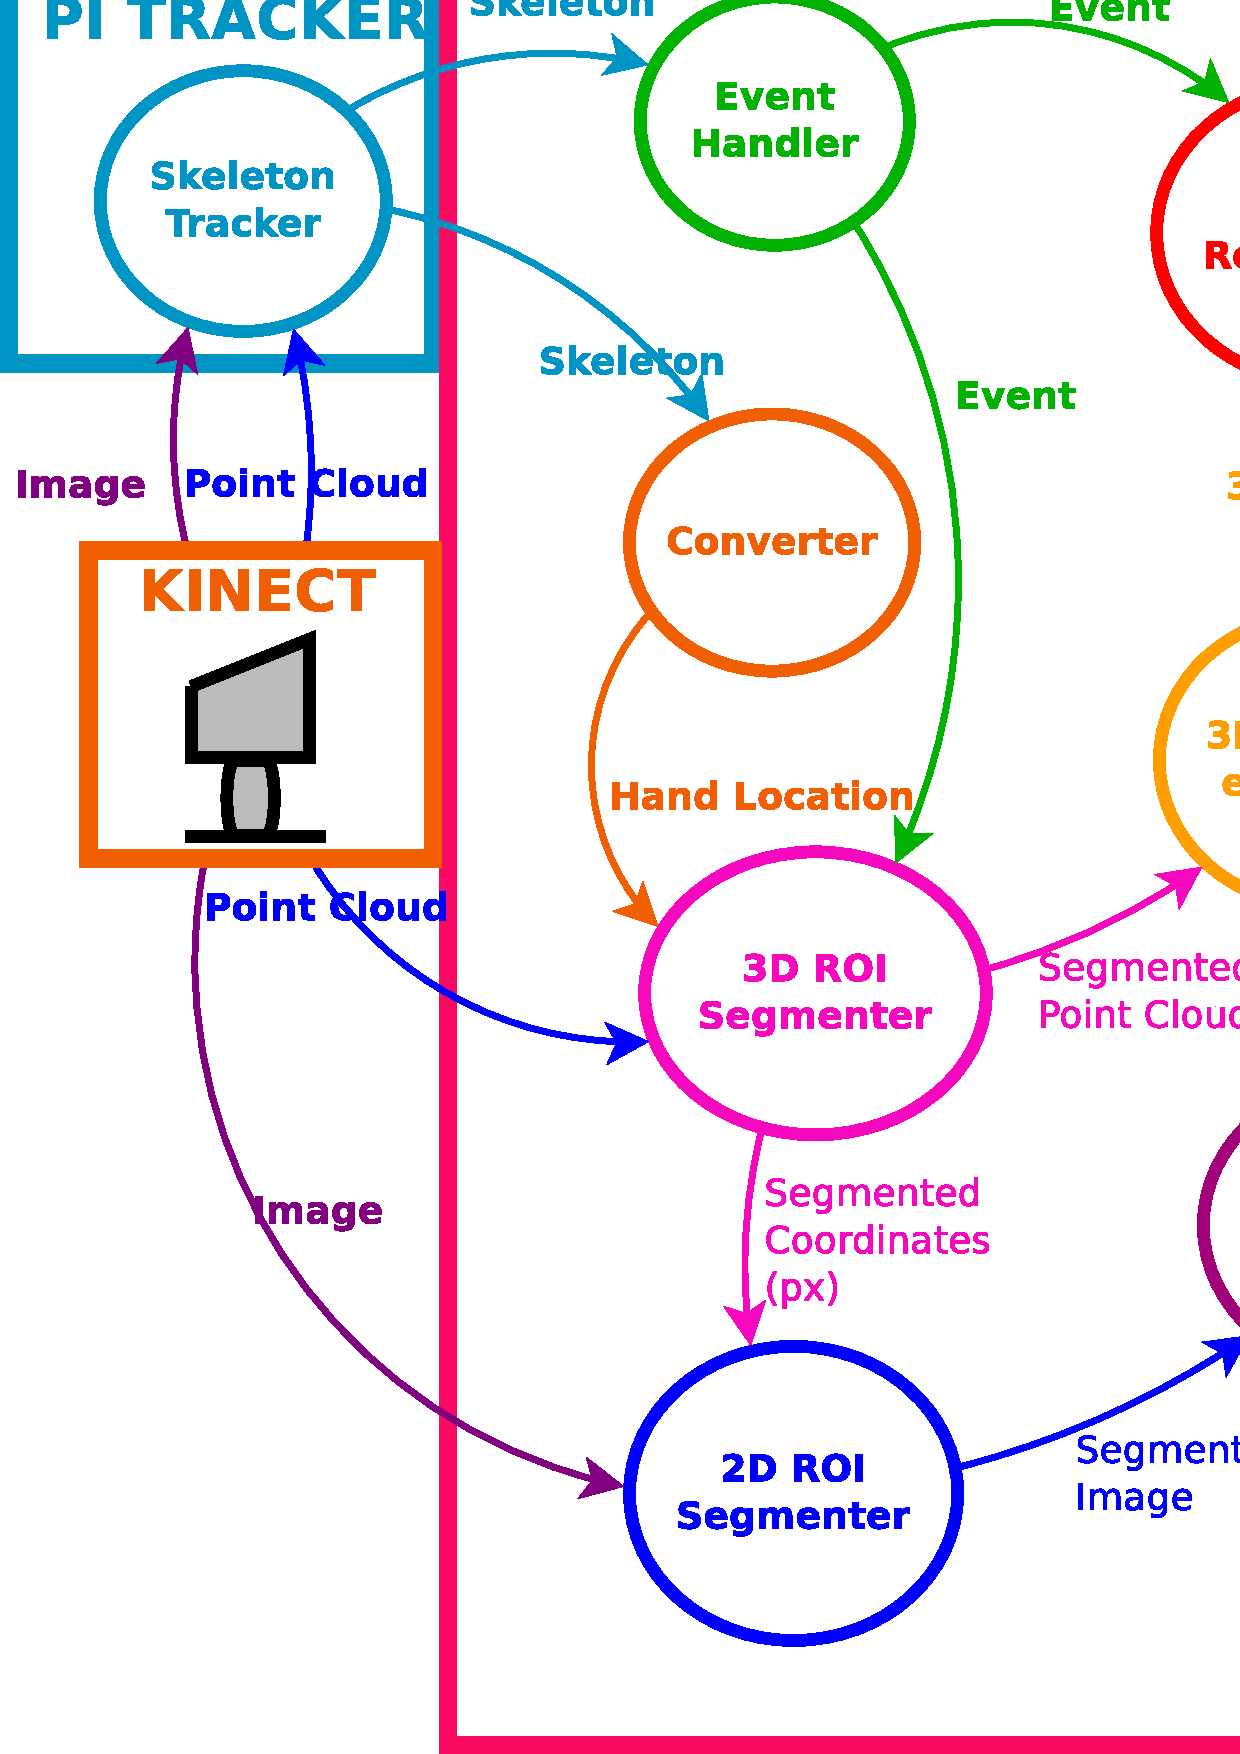
\includegraphics[scale=0.35]{img/nodes.png}
				\caption[Nodes benchmarking]{Nodes benchmarking}
				\end{center}
			\end{figure}

			The total CPU usage is lower than the 23\%, and the RAM usage of the whole software is of less than the 5\%. 
			\\


			The difference between nodes is patent in the table.
			The CPU and RAM usage varies from  0.13 to 13.34 and from 0.1 to 1.5 respectively. 
			That is, there ia a percent variation of 99\% and  93\%  in the CPU and RAM consumption in the nodes. 
			The nodes with a higher computing consumption are the ROI segmenters and the feature extractors both 2D and 3D.
			\\

			The learner recognizer node also has a higher consumption than the converter, event handler or system output nodes. 
			

		\item{\textbf{Topic Benchmarking}}\\

	\end{itemize}